\chapter{Fundamental Concepts in Graph Theory}

\section{Basic Definitions}

\begin{definition}[Graph]
  A \textit{Graph} is a set of points---called \textit{vertices}---and a set of lines---called \textit{edges}---connecting some of the vertices. Namely, 
  \begin{displaymath}
    G = (V, E)
  \end{displaymath}
  where \(V\) is the set of vertices and \(E\) is the set of edges.

  Typically, we use \(n\) to denote the number of edges and \(m\) to denote the number of edges. That is, \(n = |V| \text{ and } m = |E|\).
\end{definition}

\begin{definition}[Adjacency]
  If two vertices are connected by an edge, they are \textit{adjacent}. 
\end{definition}

\begin{definition}[Degree]
  The \textit{degree} of vertex \(v\), written \(\deg{v}\) or \(\deg(v)\), is
  the number of vertices \(v\) is adjacent to. 
\end{definition}

\begin{lemma}[Euler's Handshaking Lemma]
  The sum of the degress of the vertices of a graph is twice the number of edges. Symbolically,
  \[ \sum_{v \in V} \deg{v} = 2|E| \]
\end{lemma}

\begin{proof}
  Since each edge associates 2 vertices with each other, each edge will show up twice in the sum of degrees---once for each vertex it associates.
\end{proof}

\section{Graph Isomorphism}

Similar to the concept of isomorphism in Abstract Algebra, the concept of graph
isomorphism refers to two graphs that are the same but may be visualized 
differently or have different names for its vertices. Below, we describe its 
formal definition.

\begin{definition}[Graph Isomorphism]
  Let \(G\) and \(H\) be two graphs. Then, an \textit{isomorphism} between \(G\)
  and \(H\) is a bijection \(\phi : V(G) \to V(H)\) such that for any \(v, w \in
  V(G)\), the number of edges between \(v\) and \(w\) is the same as the number
  of edges between \(\phi(v)\) and \(\phi(w)\) in \(V(H)\). If such bijection
  exists, then we say that \(G\) is \textit{isomorphic} to \(H\). Symbolically, we write \(G \cong H\).
\end{definition}

\begin{figure}[ht]
\begin{nexample}
  Here are a few examples of isomorphic graphs.

    \begin{center}
      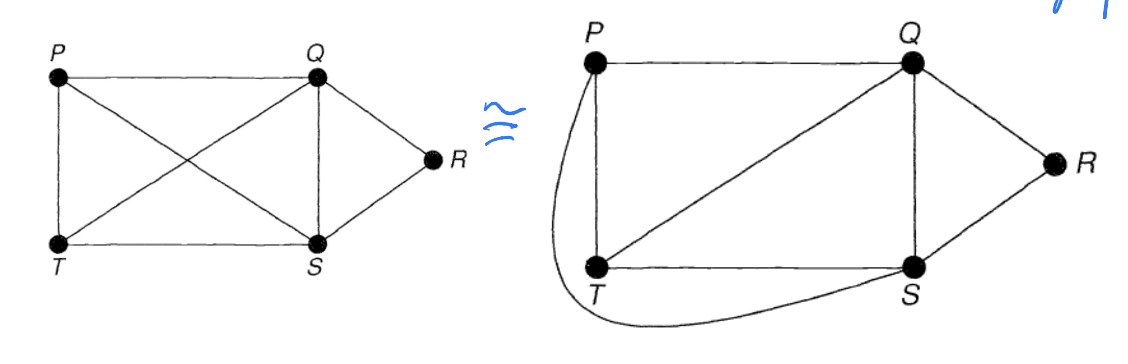
\includegraphics[width=0.69\textwidth]{figures/l01/isomorphic-graphs}
      \caption{Isomorphic Graphs}\label{fig:isomorphic-graphs}
    \end{center}

  \begin{center}
    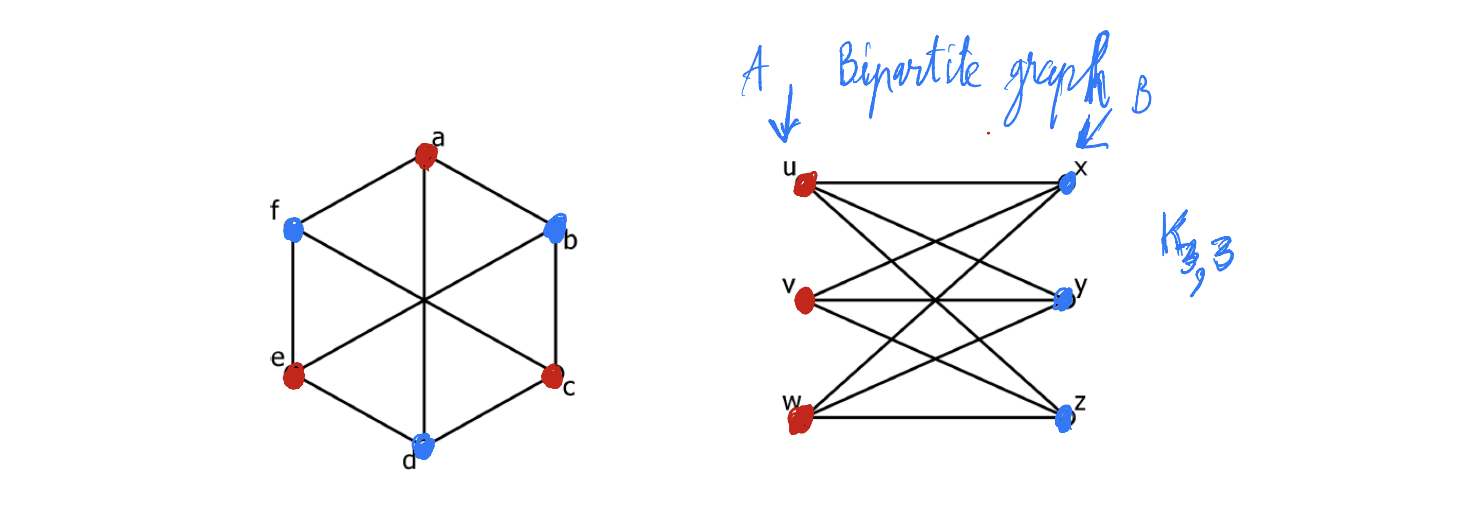
\includegraphics[width=0.69\textwidth]{figures/l01/isomorphism-example}
    \caption{Isomorphism between Two Graphs}\label{fig:isomorphism-example}
  \end{center}
\end{nexample}
\end{figure}

\begin{figure}
\begin{nexample}
  For \(n = 1, 2, 3, 4\), we will end up with 11 non-isomorphic graphs with \(n\) vertices as visualized in Figure~\ref{fig:non-isomorphic-graphs}.

    \begin{center}
      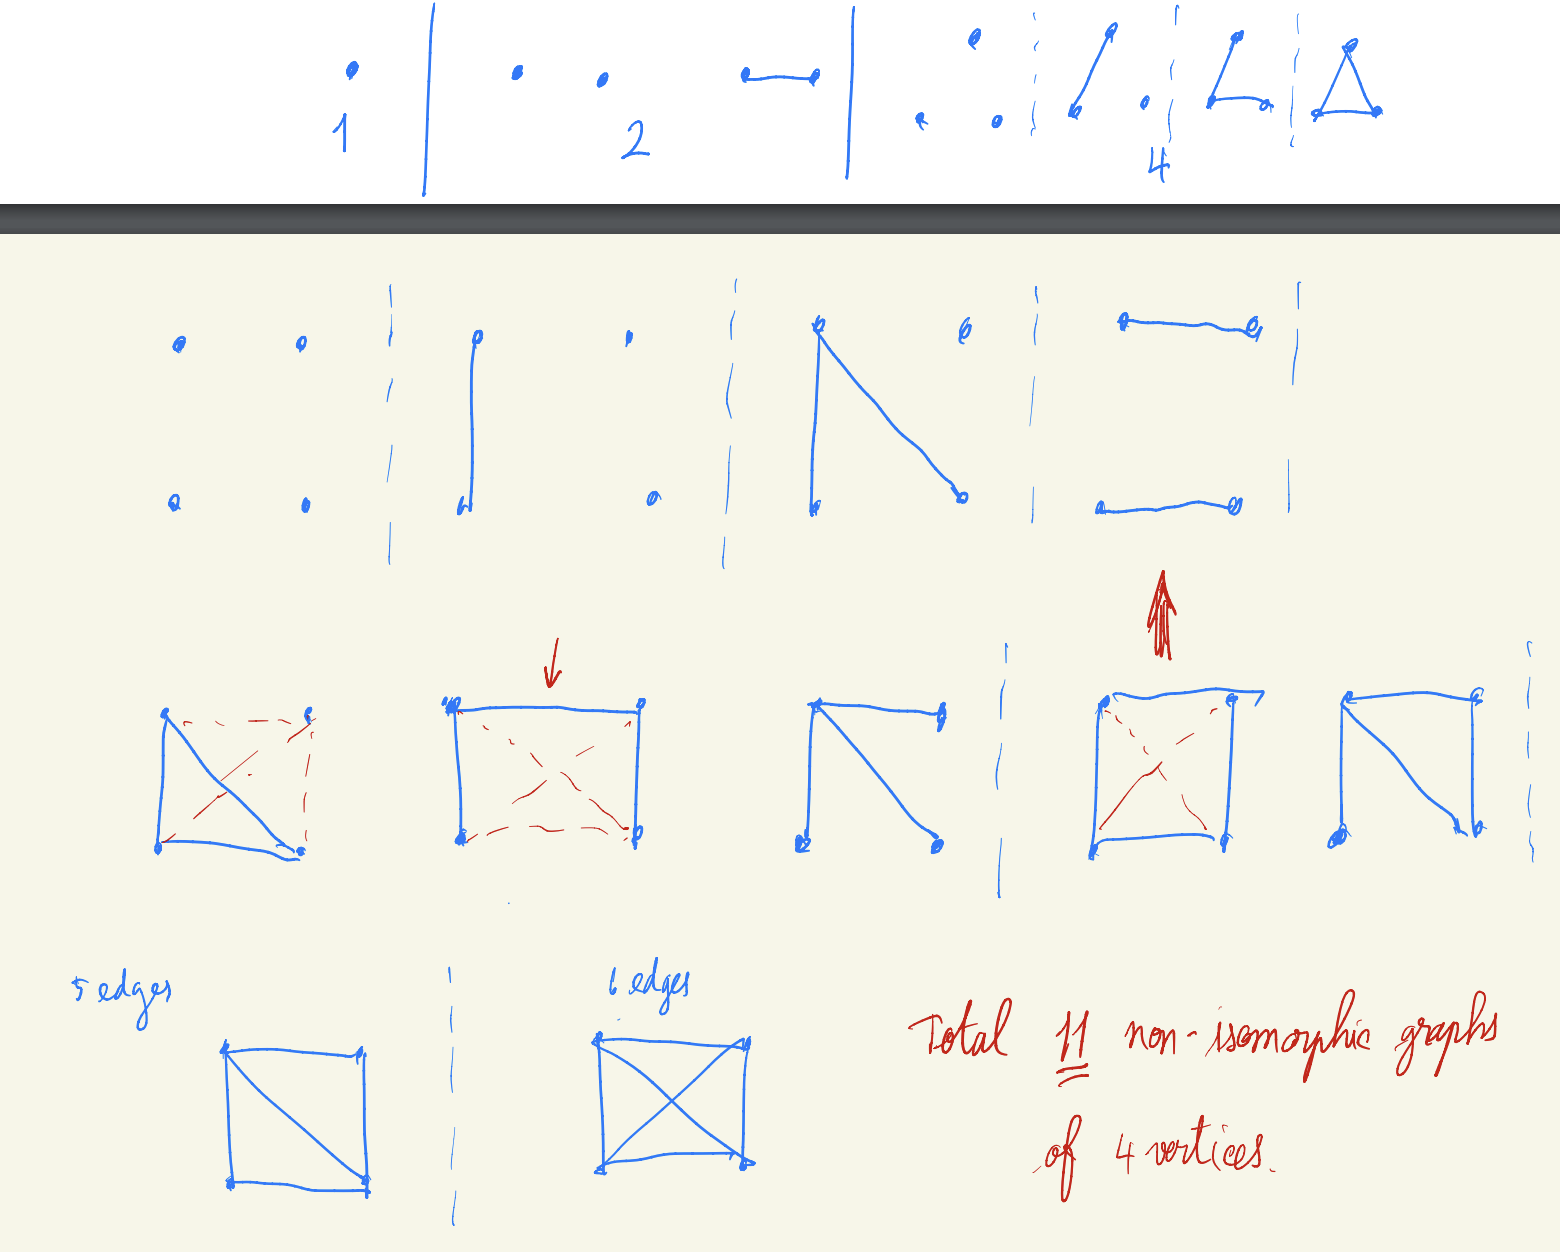
\includegraphics[width=0.69\textwidth]{figures/l01/non-isomorphic-graphs}
    \end{center}
    \caption{Non-isomorphic Graphs}\label{fig:non-isomorphic-graphs}
\end{nexample}
\end{figure}

\subsection*{Identifying Non-isomorphic Graphs}

What about identifying non-isomorphic graphs? We have a few ways:
\begin{itemize}
  \item Check \(|V|\)
  \item Check \(|E|\)
  \item Check the degrees of the vertices---\textit{the degree sequence}
  \item Check the subgraphs
    \begin{itemize}
      \item Check the length of the cycles
    \end{itemize}
  \item Show that it is impossible to come up with a bijection
\end{itemize}

\begin{figure}[ht]
\begin{nexample}
  ...
\end{nexample}
\end{figure}

\section{Subgraphs}

\begin{definition}[Subgraph]
  Let \(G\) and \(H\) be graphs. We say that \(H\) is the \textit{subgraph} of
  \(G\) if \(V(H) \subseteq V(G)\) and \(E(H) \subseteq E(G)\).
\end{definition}

\begin{definition}[Spanning Subgraphs]
  Let \(G\) and \(H\) be graphs. If \(V(H) = V(G)\) and \(E(H) \subseteq E(G)\), then we say that \(H\) is a \textit{spanning subgraph}.
\end{definition}

Notice that subgraphs includes the equal case as well. Thus, it follows that graph \(G\) is always a subgraph of itself. A \textit{proper subgraph},
however, is a subgraph of \(G\) which is not \(G\) itself. Next, we will discuss
an important type of
subgraph called the \textit{induced subgragh}.

\begin{definition}[Induced Subgraph]
  \(H\) is an \textit{induced subgraph} of \(G\) if \(V(H) \subseteq V(G)\) and \(E(H)\)
  is the set of edges in \(E(G)\) with both vertices in \(V(H)\). 

  Intuitively, we pick vertices from \(V(G)\) and we only pick edges from
  \(E(G)\) such that every edge that shows up in \(E(H)\) are associated with
  only vertices in \(V(H)\). Note that edges in \(E(H)\) does not have to
  connect every component of \(H\).
\end{definition}

\begin{figure}[ht]
\begin{nexample}
  Here are a few examples of induced subgraphs.

  \begin{center}
    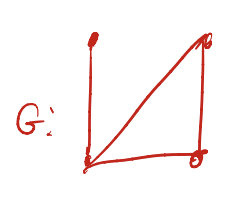
\includegraphics[width=0.25\textwidth]{figures/l01/induced-original}
    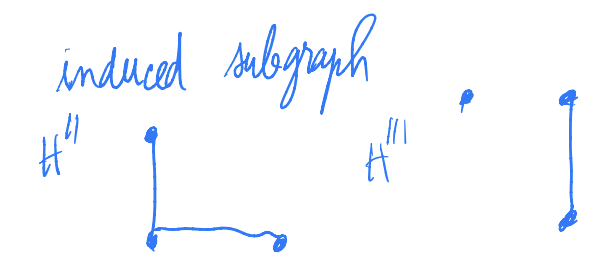
\includegraphics[width=0.45\textwidth]{figures/l01/induced-subgraph}
    \caption{Original graph \(G\) and its induced subgraphs \(H'', H'''\)}\label{fig:induced-subgraph}
  \end{center}
\end{nexample}
\end{figure}

\section{Types of Graphs}

\begin{definition}[Complete Graphs]
  \textit{Complete graphs}, often denoted \(K_n\), are graphs with \(n\) vertices and
  each vertex is connected to the rest of the vertices by precisely one edge.
  These graphs have \(\binom{n}{2}\) edges.
\end{definition}

\begin{definition}[Paths]
  The \textit{path} \(P_n\) is the (sub)graph with \(n\) distinct vertices \(v_1, v_2, ...,
  v_n\) and \(n-1\) edges where they are \((v_1, v_2), (v_2, v_3), ..., (v_{n-1}, v_n)\). Some important properties of paths are that they cannot have repeated edges and that they do not form cycles.
\end{definition}

\begin{definition}[Cycles]
  The \textit{cycle} \(C_n\) is a (sub)graph with \(n\) edges obtained from \(P_n\) by adding an
  edge between the two ends. Intuitively, it creates a polygon of \(n\) sides.
\end{definition}

An important property that paths and cycles share is that they cannot have
repeated vertices. That is, the degree of each vertex in a path or a cycle is at
most two. For the \textit{end points} of a path, the degree is exactly one.

\begin{definition}[Wheel Graphs]
  The wheel graph \(W_{n+1}\) is the graph obtained from \(C_n\) by adding one
  more vertex that connects to every vertex in \(C_n\).
\end{definition}

\begin{figure}[ht]
\begin{nexample}
  There are five \textit{platonic graphs} corresponding to the five platonic solids. This
  is shown below

  \begin{center}
    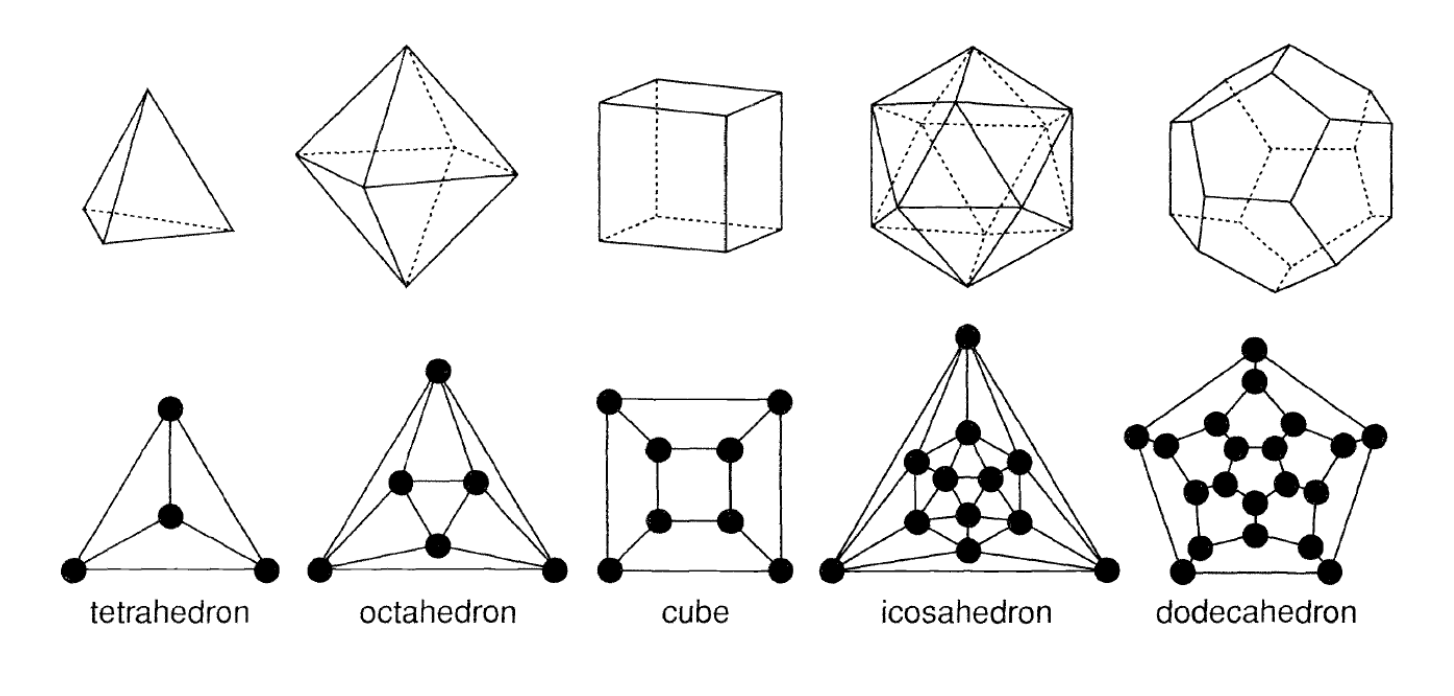
\includegraphics[width=0.95\textwidth]{figures/l01/platonic-solids}
  \end{center}
  \caption{Platonic Solids}\label{fig:l01-platonic-solids}
\end{nexample}
\end{figure}

\begin{definition}[Regular Graphs]
  A \textit{regular graph} is a graph where all vertices have the same degree. 
  Furthurmore, a \textit{\(k\)-regular graph} is a graph where all vertices have degree \(k\).
\end{definition}

\begin{definition}[Bipartite Graphs]
  A \textit{bipartite graph} is a graph where the vertices can be split into two sets
  \(V_1\) and \(V_2\) such that all edges are between \(V_1\) and \(V_2\). In
  addition, the vertices in \(V_1\) cannot have edges between themselves. Same
  goes for \(V_2\).
\end{definition}

\begin{definition}[Complete Bipartite Graphs]
  \textit{Complete bipartite graphs}, denoted \(K_{m, n}\) are bipartite graphs such that \(|V_1| = m\) and \(|V_2| = n\) and each vertex in \(V_1\) is
  connected by exactly one edge to every vertex in \(V_2\) and vice-versa. Note
  that \(K_{m, n}\) graphs have \(m \cdot n \) edges.
\end{definition}

\begin{nexample}
  Let us find the number of spanning subgraphs in the complete graph \(K_n\) and a complete bipartite graph \(K_{m, n}\).

  Notice that in the complete graph \(K_3\), there can be \(2^3 = 8\) spanning graphs.
  Similarly, in the complete subgraph \(K_4\), there can be 
  \(2^6 = 64\) spanning subgraphs. Namely, we are considering every possible
  edge based on the number of vertices that we have. Since the base graph is a complete graph, the possible edges can be derived from every possible pair of vertices. Then, for each edge, we can choose to
  either include it in the graph or not. Since there are \(\binom{n}{2}\)
  possible edges, we can conclude that there are \(2^{\binom{n}{2}}\) spanning subgraphs of \(K_n\).

  As for the complete bipartite graph, recall that a \(K_{m, n}\) graph has
  \(m \cdot n\) edges. Thus, using the same reasoning as for \(K_n\) graphs, we have \(2^{mn}\) spanning subgraphs of \(K_{m, n}\).
\end{nexample}

\begin{definition}[Simple Graphs]
  A graph \(G\) is a \textit{simple graph} if the following satisfies:
  \begin{itemize}
    \item For each pair of vertices \(v, w \in V(G)\), there is at most one edge
      between them
    \item No edge can start and end at the same vertex
  \end{itemize}
  Intuitively, this means that there can be no loops nor repeat edges.
\end{definition}

\begin{definition}[Complement Graph]
  Let \(G\) be a simple graph. The \textit{complement} of \(G\), denoted
  \(\overline{G}\), is the graph where for every pair of vertices \(v, w\), if
  \((v, w) \in E(G)\), then \((v, w) \notin E(\overline{G})\).
\end{definition}

\begin{remark}[Duality]
  Notice that, for a graph \(G\), the complement of the complement of \(G\) is
  \(G\). That is 
  \[ \overline{\overline{G}} = G \]
  This phenomenon is referred to as \textit{duality}.
\end{remark}

\begin{definition}[Connected Graphs]
  A graph is \textit{connected} if for each pair of vertices \(v, w\), there
  exists a path that joins them.
\end{definition}

\begin{figure}[ht]
\begin{nexample}
    \textit{Peterson Graphs} are \(3\)-regular graphs with 10 vertices.
   
  \begin{center}
    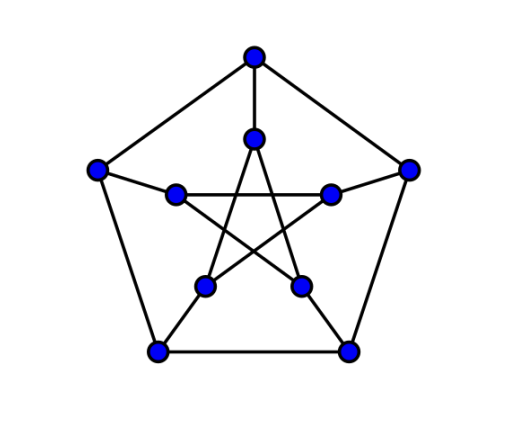
\includegraphics{figures/l01/peterson-graph}
  \end{center}
  \caption{Peterson Graph}\label{fig:l01-peterson-graph}
\end{nexample}
\end{figure}

\subsection{Relevant Theorems}

\begin{theorem}
  Let \(G\) be a simple graph. If \(G\) is disconnected, then \(\overline{G}\) is connected.
\end{theorem}

\begin{proof}
  Assume that \(G\) is disconnected. We will show that \(\overline{G}\) is
  connected. Namely, we want to show that for every vertex \(v, w \in
  V({G})\), there is a path between them in \(V(\overline{G})\). We will show
  this by case.

  \textit{Case 1.} If \(v\) and \(w\) are in different components, then there
  is no edge between them in \(E(G)\). Thus, there will be an edge between them
  in \(E(\overline{G})\).

  \textit{Case 2.} If \(v\) and \(w\) are in the same component, then we can
  pick any vertex \(u\) in any other component and make the path \(v \to u \to
  w\).
\end{proof}

\begin{definition}[Distance]
  The \textit{distance} from vertex \(u\) to vertex \(v\) is the length of the
  shortest path from \(u\) to \(v\).
\end{definition}

\begin{theorem}[Criterion for Bipartite Graphs]
  A non-trivial graph \(G\) is a bipartite graph if and only if \(G\) contains
  no odd cycles.
\end{theorem}

\begin{proof}
  First, we will show the forward direction: If \(G\) is bipartite then
  every cycle in \(G\) is even. That is, we will show that
  \(m\) is odd for every cycle \(v_0 \to
  v_1, ..., v_m \to v_0\) in \(G\). Since \(G\) is bipartite, we can separate
  the vertices into sets \(A\) and \(B\). Without loss of generality, suppose
  that \(v_0 \in A\). Then, we have \(v_1 \in B\), \(v_2 \in A\), and so on.
  Since we are considering a cycle, we must end at vertex \(v_0\). Hence,
  \(v_m\) must be in \(B\). Since all \textit{even vertices} are in \(A\) and all \textit{odd vertices} are in \(B\), we have that \(m\) is an odd number. Therefore, we can conclude that if \(G\) is bipartite, then \(G\) contains no odd cycles.

  Now, we will show the converse case: If there are no odd cycles in graph \(G\), then \(G\) is bipartite. Specifically, we will show this by contraposition. Let us assume that \(G\) is \textbf{not} bipartite. Then, we will show that \(G\) contains an odd cycle. Without loss of generality, we will assume that \(G\) is connected. Otherwise, we can consider each component of \(G\) separately. Consider the vertex \(v \in V(G)\) and put \(v\) in a set \(A\). Then, put every vertex with odd distance from \(v\) in a set \(B\) and every vertex with even distance from \(v\) in \(A\). Since \(G\) is not bipartite, there must be an edge within the set \(A\) or \(B\). Let us (informally) call this edge an \textit{inner edge}, denoted \((u, w)\).
  \begin{itemize}
    \item If the inner edge is in \(A\), we can form a cycle 
      \[ 
      C = v \to \underbrace{\cdots}_\text{even distance} \to u \to w \to \underbrace{\cdots}_\text{even distance} \to v 
    \]
      where \(C\) is odd
    \item If the inner edge is in \(B\), we can form a cycle 
      \[ 
      C = v \to \underbrace{\cdots}_\text{odd distance} \to u \to w \to \underbrace{\cdots}_\text{odd distance} \to v 
    \]
    where \(C\) is odd as well
  \end{itemize}
  Thus, we have that if the graph \(G\) is not bipartite, then there exists an
  odd cycle in \(G\). Therefore, we can conclude that if graph \(G\) contains no
  odd cycle, then \(G\) is bipartite by contrapositivity.
\end{proof}

\begin{theorem}
  Let \(r\) and \(n\) be integers with \(0 \leq r \leq n-1\). There exists an
  \(r\)-regular graph of order \(n\) if and only if at least one of \(r\) or
  \(n\) is even.
\end{theorem}

\begin{proof}
  We will first show the forward direction: If a graph is \(r\)-regular with
  order \(n\), then at least one of \(r\) or \(n\) is even. Assume to the
  contrary that both \(r\) and \(n\) are odd. Consider
  \[
  \begin{aligned}
    \sum_{v \in G} \deg{v} = \underbrace{r + r + ... + r}_{\text{\(n\) times}} =
    r \cdot n
  \end{aligned}
  \]
  Notice that this summation results in an odd number since the product of odd
  numbers is also odd. This is impossible due to the handshaking lemma since
  the sum of the degrees must be even. Thus, there can be no such graph 
  exists. Therefore, we can conclude that if a graph is \(r\)-regular with order
  \(n\), then at least one of \(r\) or \(n\) is even.

  Now, we will show the converse direction: If at least one of \(r\) or \(n\) is
  even, then there exists an \(r\)-regular graph of order \(n\). We will show
  these by case:
  \begin{itemize}
    \item \textit{Case 1: \(r\) is even.} We can arrange the \(n\) vertices into a \textit{round shape}. Then, for each \(v \in V(G)\), connect \(v\) to the \(r/2\) closest vertices counter-clockwise and \(r/2\) closest vertices clockwise. This results every \(v \in G\) having \(r\) edges, making this graph \(r\)-regular.

    \item \textit{Case 2: \(r\) is odd but \(n\) is even.} We repeat the procedure for case 1 but connects \(v\) to \(\lfloor r/2 \rfloor\) closest instead and add another edge to the \textit{opposite} vertex of \(v\) so that each vertex has degree \(r\).
  \end{itemize}
  The visualization of this proof can be seen in Figure~\ref{fig:rn-proof-viz}.
\end{proof}

\begin{figure}[ht]
  \begin{center}
    \hfill
    \begin{subfigure}{0.23\textwidth}
      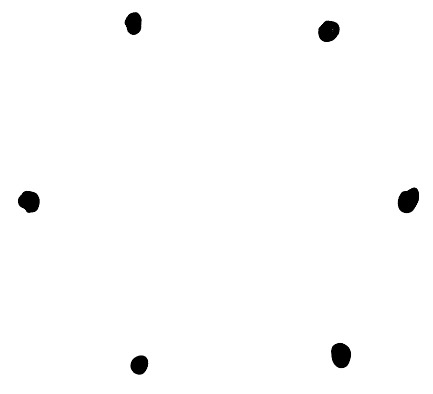
\includegraphics[width=\textwidth]{figures/l02/l02-step1}
      \caption{Round shape}
    \end{subfigure}
    \hfill
    \begin{subfigure}{0.23\textwidth}
      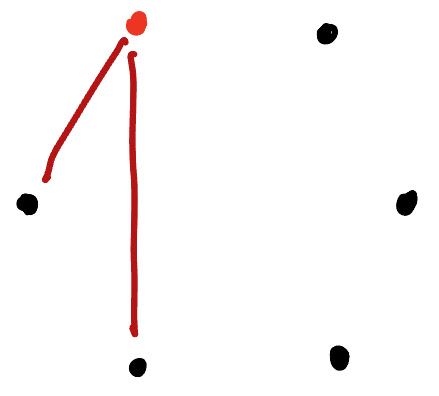
\includegraphics[width=\textwidth]{figures/l02/l02-step2}
      \caption{\(r/2\) closest CCW}
    \end{subfigure}
    \hfill
    \begin{subfigure}{0.23\textwidth}
      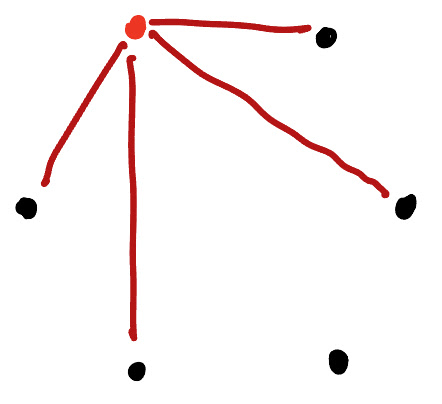
\includegraphics[width=\textwidth]{figures/l02/l02-step3}
      \caption{\(r/2\) closest CW}
    \end{subfigure}
    \hfill
    \begin{subfigure}{0.23\textwidth}
      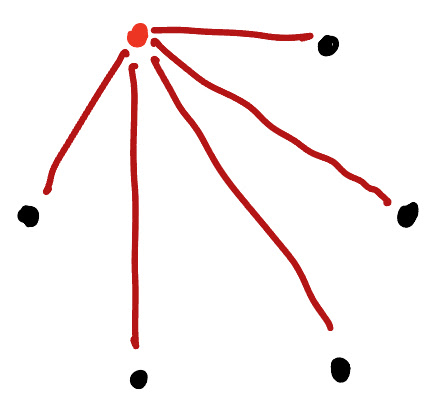
\includegraphics[width=\textwidth]{figures/l02/l02-step4}
      \caption{Opposite (when \(r\) odd)}
    \end{subfigure}
    \hfill
  \end{center}
  \caption{Visualization of proof when \(n=6, r=\{4, 5\}\)}\label{fig:rn-proof-viz}
\end{figure}

